\section{Application-level conventions}\label{sec:application_level_conventions}

\subsection{Identifier distribution}

An overview of related concepts is provided in chapter \ref{sec:basic_concepts}.

\subsubsection{Node ID}

Valid values of node ID range from 0 to 127, inclusive.

The node ID values 126 and 127 are reserved for diagnostic and debugging tools;
these node ID values should not be used in fielded systems.

\subsubsection{Port ID}

This rule is mandatory for all applications.

The subject and service identifier values are segregated into three ranges:
unregulated port identifiers that can be freely chosen by users and integrators (both fixed and non-fixed);
regulated fixed identifiers for non-standard data type definitions
that are assigned by the UAVCAN maintainers for publicly released data types;
and regulated identifiers of the standard data types that are an integral part of the UAVCAN specification.

More information on the subject of data type regulation is provided in section
\ref{sec:basic_concepts_data_type_regulation}.

The ranges are summarized in the table \ref{table:application_port_id_distribution}.
Unused gaps are reserved for future expansion of adjacent ranges.

\begin{UAVCANSimpleTable}{Port identifier distribution}{|l l X|}\label{table:application_port_id_distribution}
    Subject ID          & Service ID        & Purpose \\
    $[0, 32767]$        & $[0, 127]$        & Unregulated identifiers (both fixed and non-fixed). \\
    $[57344, 59391]$    & $[256, 319]$      & Non-standard regulated identifiers (i.e., vendor-specific). \\
    $[62804, 65535]$    & $[384, 511]$      & Standard regulated identifiers. \\
\end{UAVCANSimpleTable}

\subsection{Coordinate frames}

UAVCAN follows the conventions that are widely accepted in relevant applications.
Adherence to the coordinate frame conventions described here maximizes system compatibility and
reduces the amount of computations for conversions between incompatible coordinate systems and
representations.
It is recognized, however, that some applications may find the advised conventions unsuitable,
in which case deviations are permitted.
Any such deviations must be explicitly documented.

All coordinate systems defined in this section are right handed.
If application-specific coordinate systems are introduced, they should be right handed as well.

\begin{figure}[hbt]
    \centering
    % The source image is released under CC0, public domain, no attribution required:
    % https://commons.wikimedia.org/wiki/File:ECEF_ENU_Longitude_Latitude_relationships.svg
	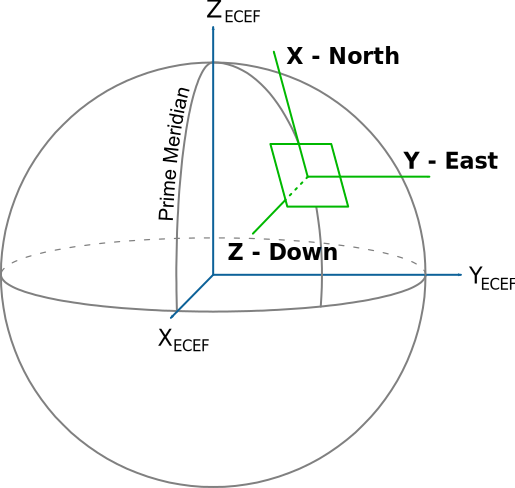
\includegraphics[width=0.45\textwidth]{application_layer/NED_ECEF}
    % The source image is released under CC0, public domain, no attribution required:
    % https://pixabay.com/en/airplane-plane-aircraft-propeller-40374/
    % The final image is drawn by me. The source Inkscape SVG file is located in the same directory.
    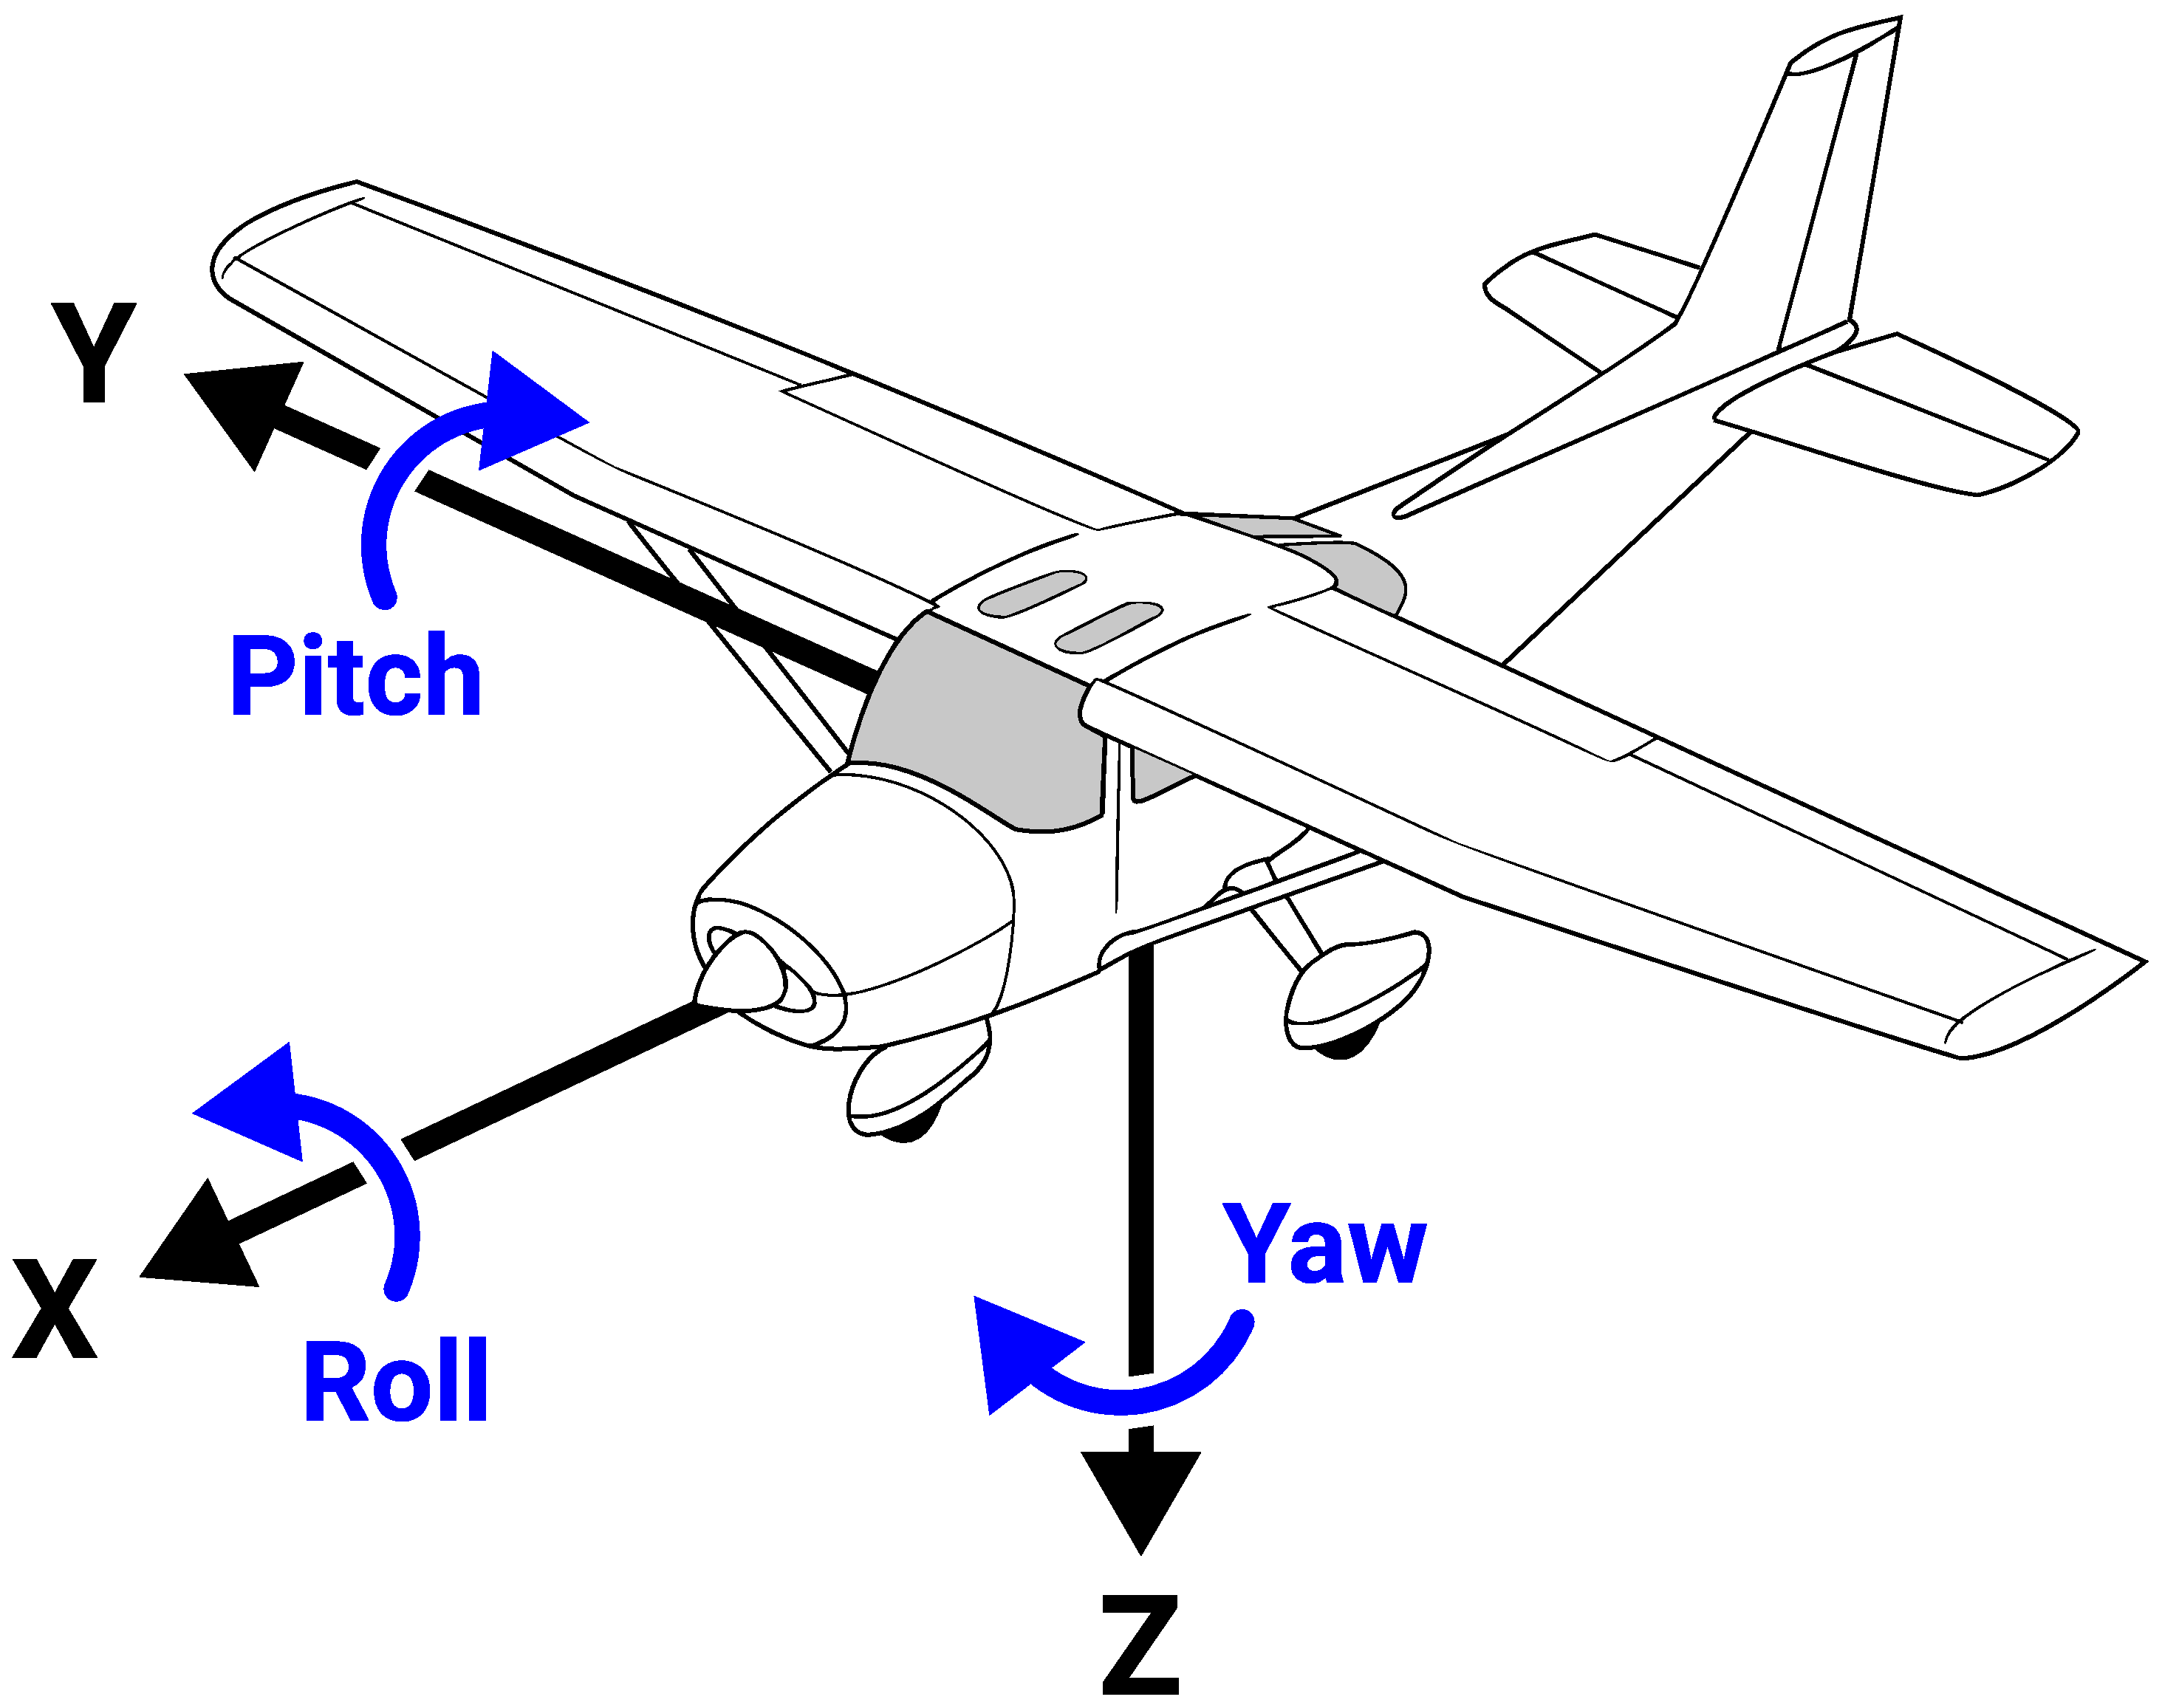
\includegraphics[width=0.45\textwidth]{application_layer/aircraft_principal_axes}
    North-East-Down (NED) frame and body frame conventions. All systems are right handed.
    \caption{
        Coordinate frame conventions.
        \label{fig:application_coordinate_frame_conventions}
    }
\end{figure}

\subsubsection{World frame}

For world fixed frames, the \emph{North-East-Down} (NED) right handed notation should be preferred.
\begin{samepage}
\begin{description}
    \item[X] --- northward;
    \item[Y] --- eastward;
    \item[Z] --- down.
\end{description}
\end{samepage}

\subsubsection{Body frame}

In relation to a body, the convention is as defined below, right handed.
This convention is widely used in aeronautic applications.
\begin{samepage}
\begin{description}
    \item[X] --- forward;
    \item[Y] --- right;
    \item[Z] --- down.
\end{description}
\end{samepage}

\subsubsection{Optical frame}

In the case of cameras, the right handed convention specified below should be preferred.
It is widely used in various applications involving computer vision systems.
\begin{samepage}
\begin{description}
    \item[X] --- right;
    \item[Y] --- down;
    \item[Z] --- towards the scene along the optical axis.
\end{description}
\end{samepage}

\subsection{Rotation representation}

All applications should represent rotations using quaternions with the elements ordered as follows\footnote{%
    Assuming $w + x\boldsymbol{i} + y\boldsymbol{j} + z\boldsymbol{k}$.
}: W, X, Y, Z.
Other forms of rotation representations should be avoided.

Angular velocities should be represented using a right handed fixed axis (extrinsic) convention:
X (roll), Y (pitch), Z (yaw).

\begin{remark}
    Quaternions are considered to offer the optimal trade-off between bandwidth efficiency,
    computation complexity, and explicitness:
    \begin{itemize}
        \item Euler angles are not self-contained, requiring applications to agree on a particular
        convention beforehand; such convention would be difficult to establish considering different
        demands of various use cases.

        \item Euler angles and fixed axis rotations typically cannot be used for computations directly
        due to angular interpolation issues and singularities; thus, in order to make use of such
        representations, one often has to convert them to a different form (e.g., quaternion);
        such conversions are relatively computationally heavy.

        \item Rotation matrices are highly redundant.
    \end{itemize}
\end{remark}

\subsection{Matrix representation}

\subsubsection{General}

Matrices should be represented as flat arrays in the row-major order.

\begin{remark}
    $
    \begin{bmatrix}
        x_{11} & x_{12} & x_{13} \\
        x_{21} & x_{22} & x_{23} \\
    \end{bmatrix} \rightarrow \left(x_{11}, x_{12}, x_{13}, x_{21}, x_{22}, x_{23}\right)
    $
\end{remark}

\subsubsection{Square matrices}

There are standard compressed representations of an $n \times n$ square matrix.

An array of size $n^2$ represents a full square matrix.
This is equivalent to the general case reviewed above.

An array of $\frac{(1 + n) n}{2}$ elements represents a symmetric matrix,
where array members represent the elements of the upper-right triangle arranged in the row-major order.
\begin{remark}
    $
    \begin{bmatrix}
        a & b & c \\
        b & d & e \\
        c & e & f \\
    \end{bmatrix} \rightarrow \left(a, b, c, d, e, f\right)
    $

    This form is well-suited for covariance matrix representation.
\end{remark}

An array of $n$ elements represents a diagonal matrix,
where an array member at position $i$ (where $i=1$ for the first element)
represents the matrix element $x_{i, i}$ (where $x_{1, 1}$ is the upper-left element).
\begin{remark}
    $
    \begin{bmatrix}
        a & 0 & 0 \\
        0 & b & 0 \\
        0 & 0 & c \\
    \end{bmatrix} \rightarrow \left(a, b, c\right)
    $
\end{remark}

An array of one element represents a scalar matrix.
\begin{remark}
    $
    \begin{bmatrix}
        a & 0 & 0 \\
        0 & a & 0 \\
        0 & 0 & a \\
    \end{bmatrix} \rightarrow a
    $
\end{remark}

An empty array represents a zero matrix.

\subsubsection{Covariance matrices}

A zero covariance matrix represents an unknown covariance\footnote{%
    As described above, an empty array represents a zero matrix,
    from which follows that an empty array represents unknown covariance.
}.

Infinite variance means that the associated value is undefined.

\subsection{Physical quantity representation}

All units should be SI\footnote{International System of Units.} units (base or derived).
Usage of any other units is strongly discouraged.

When defining data types, fields and constants that represent unscaled quantities in SI units
should not have suffixes indicating the unit, since that would be redundant.

On the other hand, fields and constants that contain quantities in
non-SI units\footnote{E.g., degree Celsius instead of kelvin.}
or scaled SI units\footnote{E.g., microsecond instead of second.}
should be suffixed with the standard abbreviation of the unit\footnote{E.g., kg for kilogram, J for joule.}
and its metric prefix\footnote{E.g., M for mega, n for nano.}
(if any), maintaining the proper letter case of the abbreviation.
In other words, the letter case of the suffix is independent of the letter case of
the attribute it is attached to.

Scaling coefficients should not be chosen arbitrarily;
instead, the choice should be limited to the standard metric prefixes defined by the
International System of Units.

All standard metric prefixes have well-defined abbreviations that are constructed from ASCII characters,
except for one: the micro prefix is abbreviated as a Greek letter ``\textmu{}'' (mu).
When defining data types, ``\textmu{}'' should be replaced with the lowercase Latin letter ``u''.

Irrespective of the suffix, it is recommended to always specify units for every field in the comments.

\begin{remark}
\begin{minted}{python}
float16 temperature           # [kelvin] Suffix not needed because an unscaled SI unit is used here.

uint24 delay_us               # [microsecond] Scaled SI unit, suffix is required. Mu replaced with "u".
uint24 MAX_DELAY_us = 600000  # [microsecond] The case of the suffix must not be forced to avoid confusion.

float32 kinetic_energy_GJ     # [gigajoule] Notice the letter case.

float16 estimated_charge_mAh  # [milliampere hour] Scaled non-SI unit. Highly discouraged (use coulomb).
float16 MAX_CHARGE_mAh = 1e4  # [milliampere hour] Notice the letter case.
\end{minted}
\end{remark}

\subsection{DSDL practices}

\subsubsection{Optional value representation}

Data structures may include optional fields that are not necessarily always populated.

The recommended approach for representing optional fields
is to use dynamic arrays with the capacity of one element,
prefixed with padding bits as necessary to retain byte alignment.

Alternatively, such one-element dynamic arrays can be replaced with two-field unions,
where the first field is empty and the second field contains the desired optional field.
The described layout is bit-compatible with the one-element array described above,
provided that the fields are not swapped.

Floating point fields may be assigned the value of not-a-number (NaN) per IEEE 754
to indicate that the value is not provided;
however, this pattern is discouraged because some nodes may not support IEEE 754 NaN values internally,
the value would still have to be transferred over the bus even if not populated,
and special case values undermine type safety.

\begin{remark}
Array-based optional field:
\begin{minted}{python}
void7                           # It is recommended to ensure byte alignment
MyType[<=1] optional_field
\end{minted}
Union-based optional field:
\begin{minted}{python}
@union
uavcan.primitive.Empty none     # Represents lack of value, unpopulated field
MyType some                     # The field of interest; field ordering is important
\end{minted}
The defined above union can be used as follows (suppose it is named \verb|MaybeMyType|):
\begin{minted}{python}
void7                           # It is recommended to ensure byte alignment
MaybeMyType optional_field
\end{minted}
The shown approaches are mutually bit-compatible.
\end{remark}

\subsubsection{Bit flag representation}

The recommended approach to define a set of flags is to define a dedicated \verb|bool|-typed field for each.
Representations based on an integer sum of powers of two\footnote{Which are popular in programming.}
are discouraged due to their poor readability and maintainability.

\begin{remark}
Recommended approach:
\begin{minted}{python}
void5
bool flag_foo
bool flag_bar
bool flag_baz
\end{minted}
Not recommended:
\begin{minted}{python}
uint8 flags             # Not recommended
uint8 FLAG_BAZ = 1
uint8 FLAG_BAR = 2
uint8 FLAG_FOO = 4
\end{minted}
\end{remark}
